% Options for packages loaded elsewhere
\PassOptionsToPackage{unicode}{hyperref}
\PassOptionsToPackage{hyphens}{url}
%
\documentclass[
  12pt,
  a4paper,
  DIV=11,
  numbers=noendperiod]{scrreprt}

\usepackage{amsmath,amssymb}
\usepackage{setspace}
\usepackage{iftex}
\ifPDFTeX
  \usepackage[T1]{fontenc}
  \usepackage[utf8]{inputenc}
  \usepackage{textcomp} % provide euro and other symbols
\else % if luatex or xetex
  \usepackage{unicode-math}
  \defaultfontfeatures{Scale=MatchLowercase}
  \defaultfontfeatures[\rmfamily]{Ligatures=TeX,Scale=1}
\fi
\usepackage{lmodern}
\ifPDFTeX\else  
    % xetex/luatex font selection
\fi
% Use upquote if available, for straight quotes in verbatim environments
\IfFileExists{upquote.sty}{\usepackage{upquote}}{}
\IfFileExists{microtype.sty}{% use microtype if available
  \usepackage[]{microtype}
  \UseMicrotypeSet[protrusion]{basicmath} % disable protrusion for tt fonts
}{}
\usepackage{xcolor}
\setlength{\emergencystretch}{3em} % prevent overfull lines
\setcounter{secnumdepth}{5}
% Make \paragraph and \subparagraph free-standing
\ifx\paragraph\undefined\else
  \let\oldparagraph\paragraph
  \renewcommand{\paragraph}[1]{\oldparagraph{#1}\mbox{}}
\fi
\ifx\subparagraph\undefined\else
  \let\oldsubparagraph\subparagraph
  \renewcommand{\subparagraph}[1]{\oldsubparagraph{#1}\mbox{}}
\fi


\providecommand{\tightlist}{%
  \setlength{\itemsep}{0pt}\setlength{\parskip}{0pt}}\usepackage{longtable,booktabs,array}
\usepackage{calc} % for calculating minipage widths
% Correct order of tables after \paragraph or \subparagraph
\usepackage{etoolbox}
\makeatletter
\patchcmd\longtable{\par}{\if@noskipsec\mbox{}\fi\par}{}{}
\makeatother
% Allow footnotes in longtable head/foot
\IfFileExists{footnotehyper.sty}{\usepackage{footnotehyper}}{\usepackage{footnote}}
\makesavenoteenv{longtable}
\usepackage{graphicx}
\makeatletter
\def\maxwidth{\ifdim\Gin@nat@width>\linewidth\linewidth\else\Gin@nat@width\fi}
\def\maxheight{\ifdim\Gin@nat@height>\textheight\textheight\else\Gin@nat@height\fi}
\makeatother
% Scale images if necessary, so that they will not overflow the page
% margins by default, and it is still possible to overwrite the defaults
% using explicit options in \includegraphics[width, height, ...]{}
\setkeys{Gin}{width=\maxwidth,height=\maxheight,keepaspectratio}
% Set default figure placement to htbp
\makeatletter
\def\fps@figure{htbp}
\makeatother

\KOMAoption{captions}{tableheading}
\usepackage{indentfirst}
\usepackage{float}
\floatplacement{figure}{H}
\usepackage{libertine}
\makeatletter
\makeatother
\makeatletter
\makeatother
\makeatletter
\@ifpackageloaded{caption}{}{\usepackage{caption}}
\AtBeginDocument{%
\ifdefined\contentsname
  \renewcommand*\contentsname{Содержание}
\else
  \newcommand\contentsname{Содержание}
\fi
\ifdefined\listfigurename
  \renewcommand*\listfigurename{Список иллюстраций}
\else
  \newcommand\listfigurename{Список иллюстраций}
\fi
\ifdefined\listtablename
  \renewcommand*\listtablename{Список таблиц}
\else
  \newcommand\listtablename{Список таблиц}
\fi
\ifdefined\figurename
  \renewcommand*\figurename{Рисунок}
\else
  \newcommand\figurename{Рисунок}
\fi
\ifdefined\tablename
  \renewcommand*\tablename{Таблица}
\else
  \newcommand\tablename{Таблица}
\fi
}
\@ifpackageloaded{float}{}{\usepackage{float}}
\floatstyle{ruled}
\@ifundefined{c@chapter}{\newfloat{codelisting}{h}{lop}}{\newfloat{codelisting}{h}{lop}[chapter]}
\floatname{codelisting}{Список}
\newcommand*\listoflistings{\listof{codelisting}{Листинги}}
\makeatother
\makeatletter
\@ifpackageloaded{caption}{}{\usepackage{caption}}
\@ifpackageloaded{subcaption}{}{\usepackage{subcaption}}
\makeatother
\makeatletter
\@ifpackageloaded{tcolorbox}{}{\usepackage[skins,breakable]{tcolorbox}}
\makeatother
\makeatletter
\@ifundefined{shadecolor}{\definecolor{shadecolor}{rgb}{.97, .97, .97}}
\makeatother
\makeatletter
\makeatother
\makeatletter
\makeatother
\ifLuaTeX
\usepackage[bidi=basic]{babel}
\else
\usepackage[bidi=default]{babel}
\fi
\babelprovide[main,import]{russian}
\babelprovide[import]{english}
% get rid of language-specific shorthands (see #6817):
\let\LanguageShortHands\languageshorthands
\def\languageshorthands#1{}
\ifLuaTeX
  \usepackage{selnolig}  % disable illegal ligatures
\fi
\usepackage[backend=biber,langhook=extras,autolang=other*]{biblatex}
\addbibresource{bib/cite.bib}
\usepackage{csquotes}
\IfFileExists{bookmark.sty}{\usepackage{bookmark}}{\usepackage{hyperref}}
\IfFileExists{xurl.sty}{\usepackage{xurl}}{} % add URL line breaks if available
\urlstyle{same} % disable monospaced font for URLs
\hypersetup{
  pdflang={ru-RU},
  hidelinks,
  pdfcreator={LaTeX via pandoc}}

\author{}
\date{}

\begin{document}
\ifdefined\Shaded\renewenvironment{Shaded}{\begin{tcolorbox}[enhanced, interior hidden, breakable, sharp corners, borderline west={3pt}{0pt}{shadecolor}, frame hidden, boxrule=0pt]}{\end{tcolorbox}}\fi

\renewcommand*\contentsname{Содержание}
{
\setcounter{tocdepth}{1}
\tableofcontents
}
\listoffigures
\listoftables
\setstretch{1.5}
\hypertarget{ux43eux431ux43dux430ux440ux443ux436ux435ux43dux438ux435-ux443ux44fux437ux432ux438ux43cux43eux441ux442ux435ux439}{%
\chapter{Обнаружение
уязвимостей}\label{ux43eux431ux43dux430ux440ux443ux436ux435ux43dux438ux435-ux443ux44fux437ux432ux438ux43cux43eux441ux442ux435ux439}}

Инциденты будут детектироваться с помощью ViPNet IDS NS.

\hypertarget{ux43eux431ux43dux430ux440ux443ux436ux435ux43dux438ux435-ux43fux435ux440ux432ux43eux439-ux443ux44fux437ux432ux438ux43cux43eux441ux442ux438}{%
\section{Обнаружение первой
уязвимости}\label{ux43eux431ux43dux430ux440ux443ux436ux435ux43dux438ux435-ux43fux435ux440ux432ux43eux439-ux443ux44fux437ux432ux438ux43cux43eux441ux442ux438}}

\begin{enumerate}
\def\labelenumi{\arabic{enumi}.}
\tightlist
\item
  Внутренний нарушитель подбирает пароль на файловый сервер и меняет
  существующий на сервере файл другим файлом с backdoor (дефектом
  алгоритма).
\item
  Пользователь Dev-1 загружает и запускает файл с backdoor.
\item
  Внутренний нарушитель получает контроль над компьютером пользователя
  Dev-1 и загружает скрипт для похищения учетных данных из браузера.
  Запускает данный скрипт и получает логин\пароль к Redmine.
\end{enumerate}

Для обраружения актуальной подозрительной активности пользуемся
фильтрами по дате, времени и важности (рис.~\ref{fig-012}).

\begin{figure}

{\centering 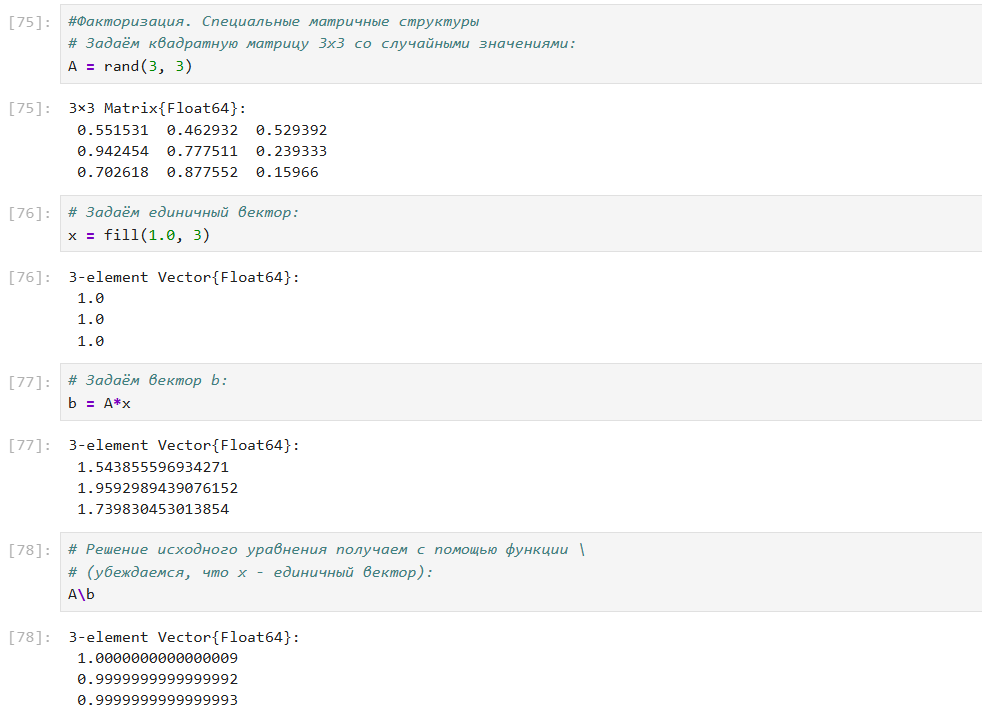
\includegraphics[width=0.7\textwidth,height=\textheight]{image/12.png}

}

\caption{\label{fig-012}Установка фильтров}

\end{figure}

Промотав в самое начало мы можем видеть создание исполняемого файла
(рис.~\ref{fig-013}), а также непосредственно событие, отвечающее за
часть атаки, запускающую код для извлечения информации
(рис.~\ref{fig-014}).

\begin{figure}

{\centering 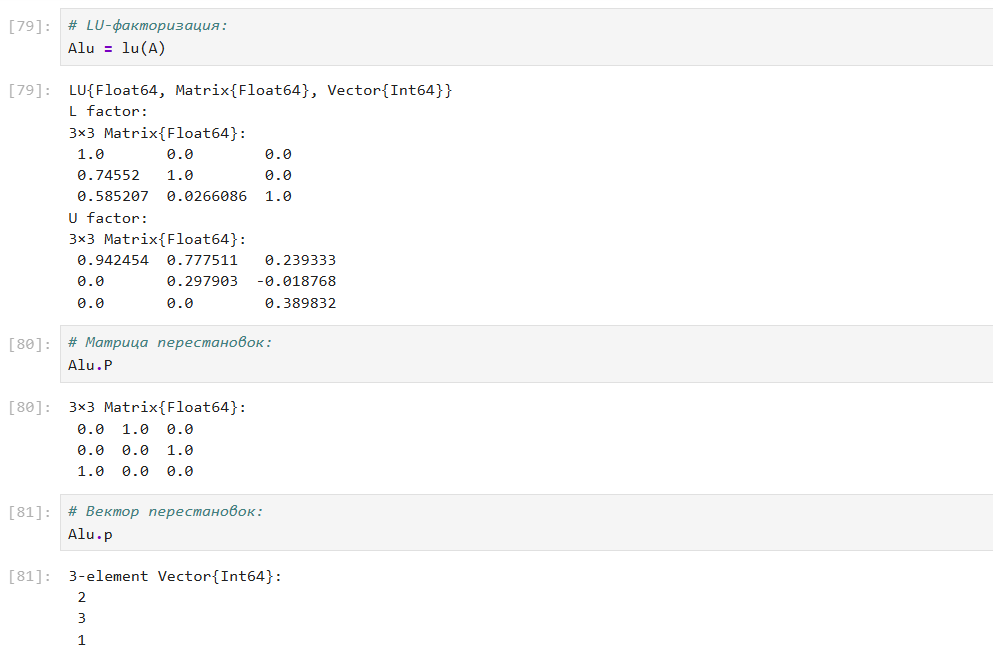
\includegraphics[width=0.7\textwidth,height=\textheight]{image/13.png}

}

\caption{\label{fig-013}Создание файла}

\end{figure}

\begin{figure}

{\centering 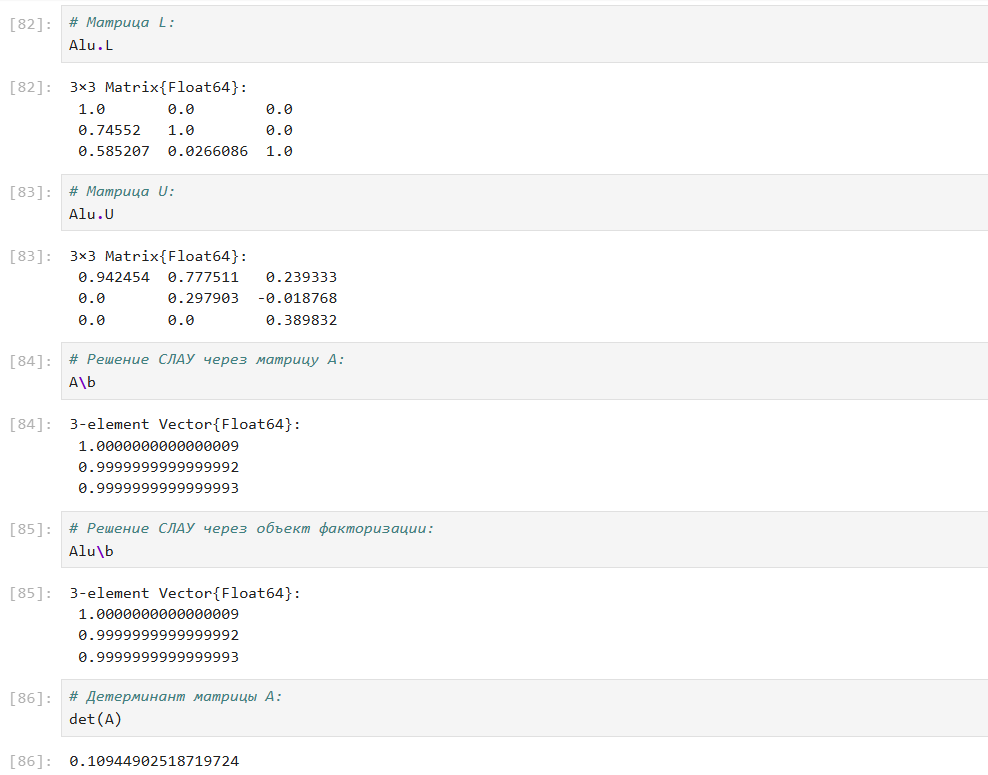
\includegraphics[width=0.7\textwidth,height=\textheight]{image/14.png}

}

\caption{\label{fig-014}Правило обнаруживающее вторичную часть атаки}

\end{figure}

Добавляем карточку для первой уязвимости (\textbf{?@fig-015}) и для
инцидента соответственно (\textbf{?@fig-016}).

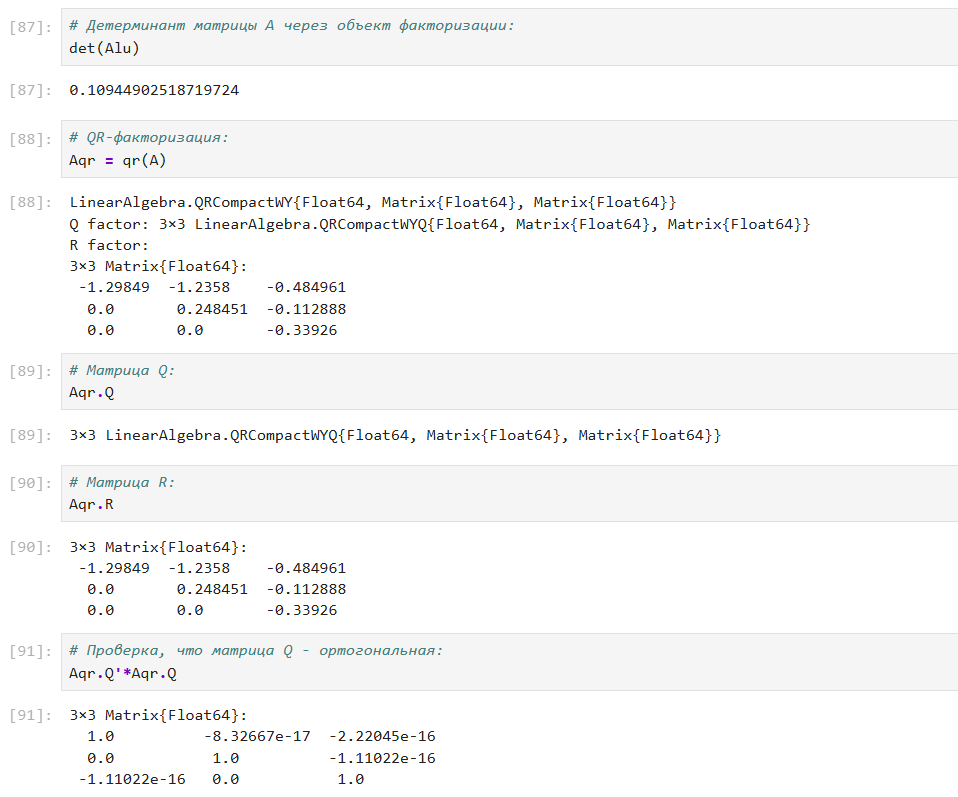
\includegraphics[width=0.7\textwidth,height=\textheight]{image/15.png}
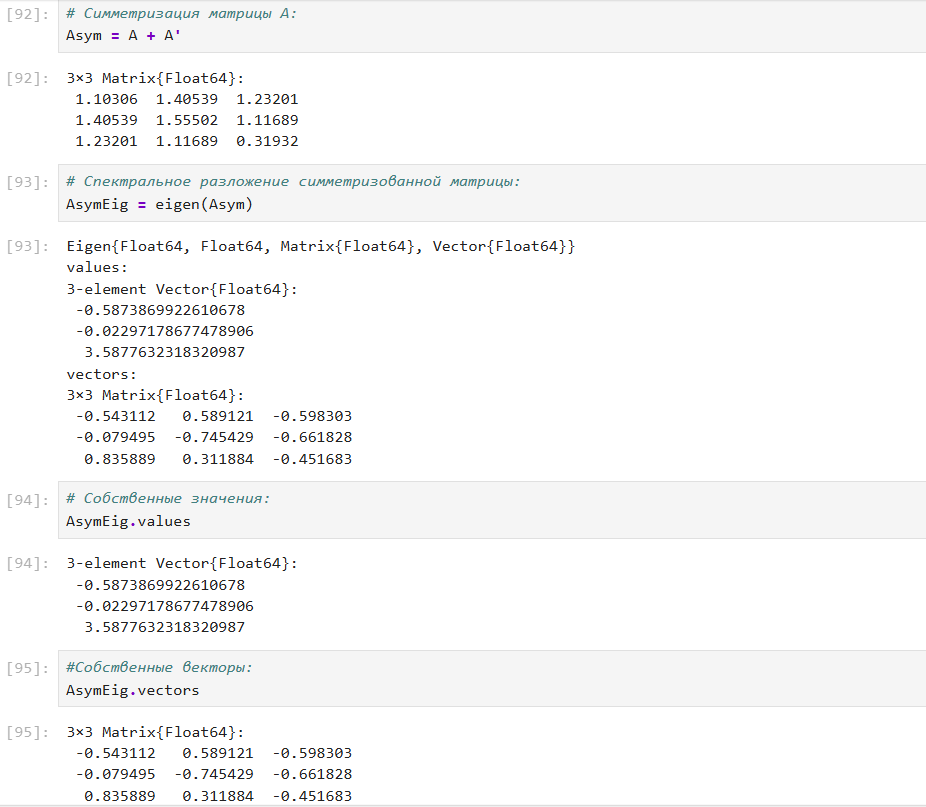
\includegraphics[width=0.7\textwidth,height=\textheight]{image/16.png}

\hypertarget{ux43eux431ux43dux430ux440ux443ux436ux435ux43dux438ux435-ux432ux442ux43eux440ux43eux439-ux443ux44fux437ux432ux438ux43cux43eux441ux442ux438}{%
\section{Обнаружение второй
уязвимости}\label{ux43eux431ux43dux430ux440ux443ux436ux435ux43dux438ux435-ux432ux442ux43eux440ux43eux439-ux443ux44fux437ux432ux438ux43cux43eux441ux442ux438}}

\begin{enumerate}
\def\labelenumi{\arabic{enumi}.}
\setcounter{enumi}{3}
\tightlist
\item
  Внутренний нарушитель проводит атаку stored XSS для включения на
  Redmine сервере REST API. Вредоносный код записывается на Wikiстраницу
  проекта Dev1. Получив доступ к консоли администратора, внутренний
  нарушитель создает нового пользователя Redmine с правами
  администратора.
\item
  Внутренний нарушитель ожидает, когда администратор просмотрит страницу
  с внедренным вредоносным кодом.
\end{enumerate}

Видим событие, отвечающее за идентифицируемую уязвимость
(рис.~\ref{fig-017}).

\begin{figure}

{\centering 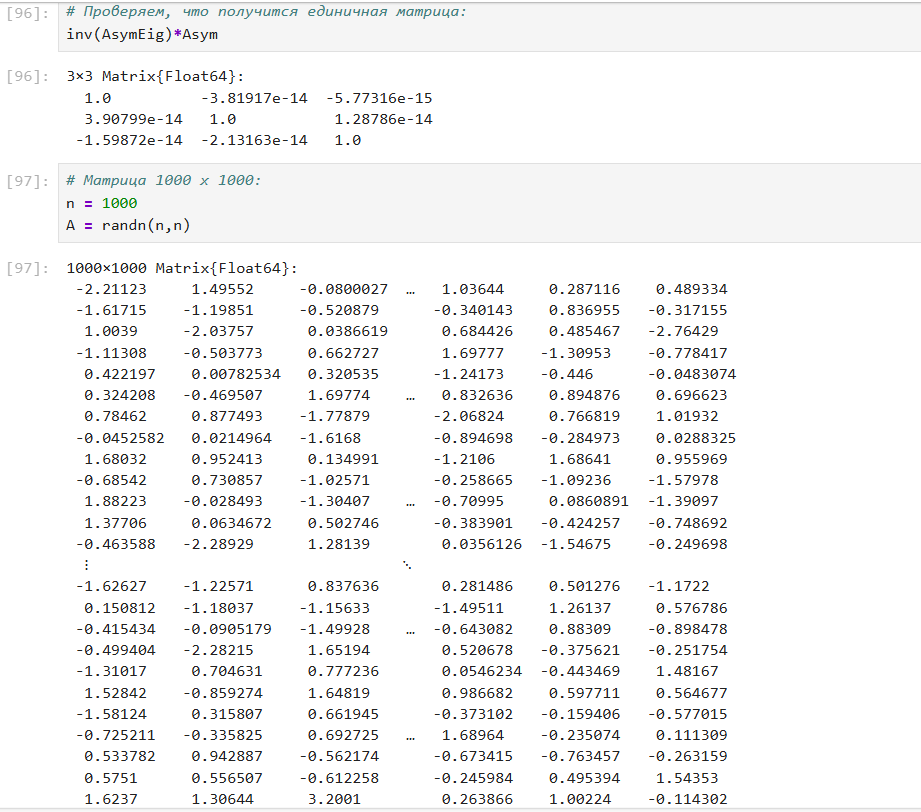
\includegraphics[width=0.7\textwidth,height=\textheight]{image/17.png}

}

\caption{\label{fig-017}Обнаруженное событие}

\end{figure}

Составляем карточку уязвимости (\textbf{?@fig-018}), общее описание и
рекомендации можно найти на сайте AMTIP (\textbf{?@fig-019}).

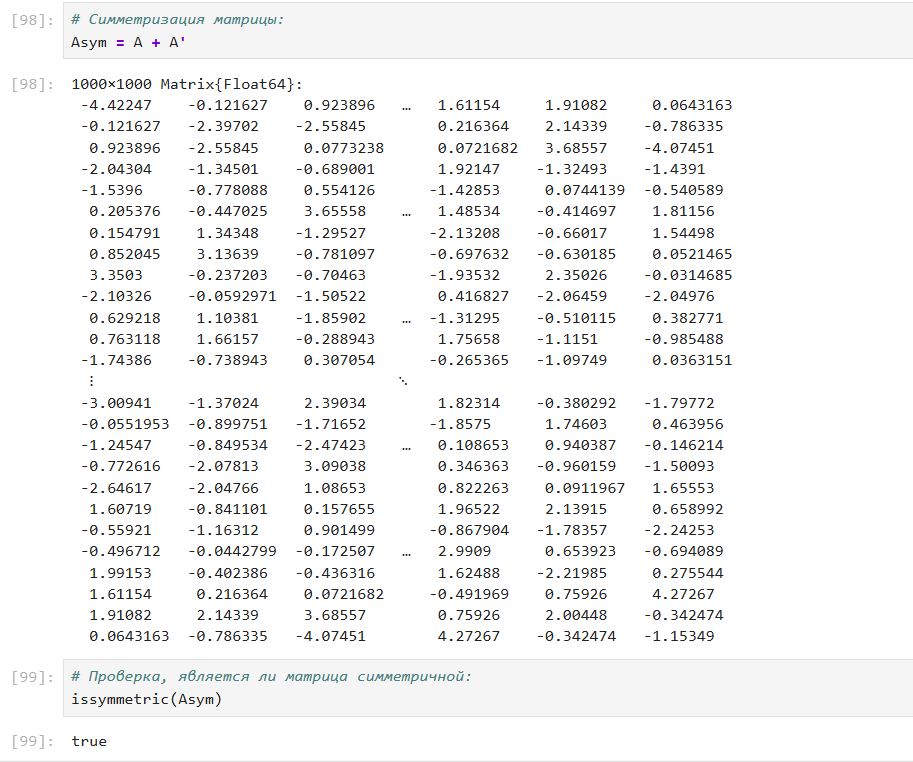
\includegraphics[width=0.7\textwidth,height=\textheight]{image/18.png}
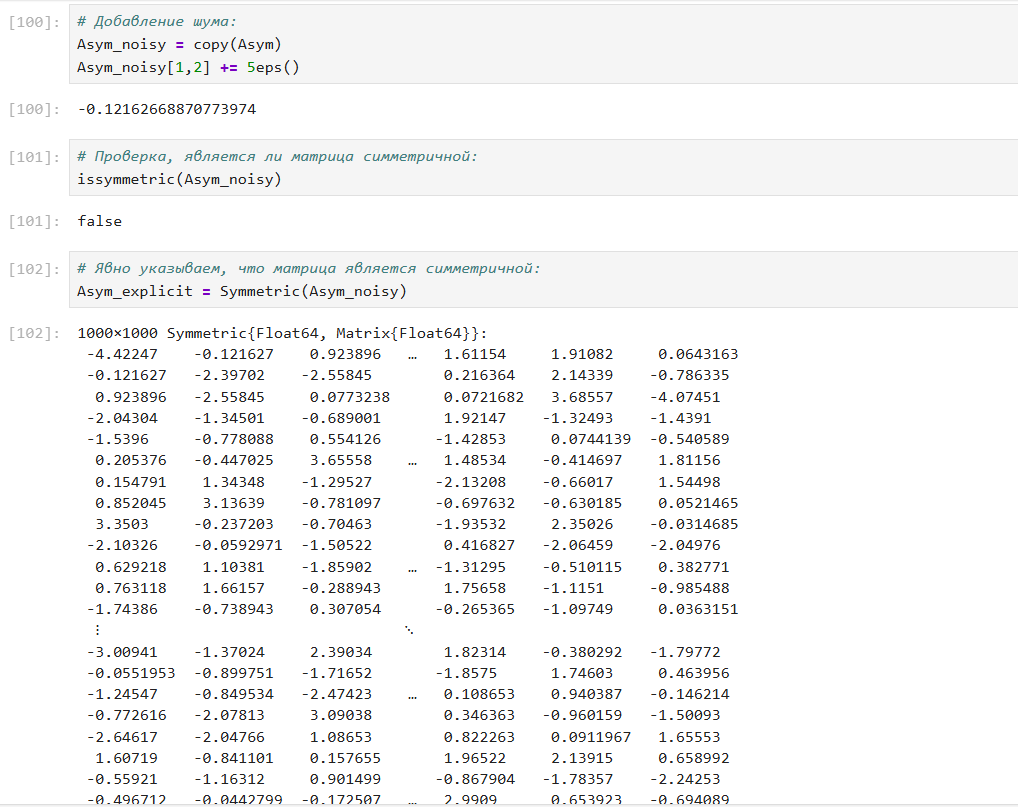
\includegraphics[width=0.7\textwidth,height=\textheight]{image/19.png}

Заходим с удаленного рабочего стола на redmin, переходим в проект DEV1
во вкладку wiki и видем, что включен REST API, а также в коде
упоминается пользователь с именем hacker (\textbf{?@fig-020}), он также
есть и в списках пользователей (\textbf{?@fig-021}).

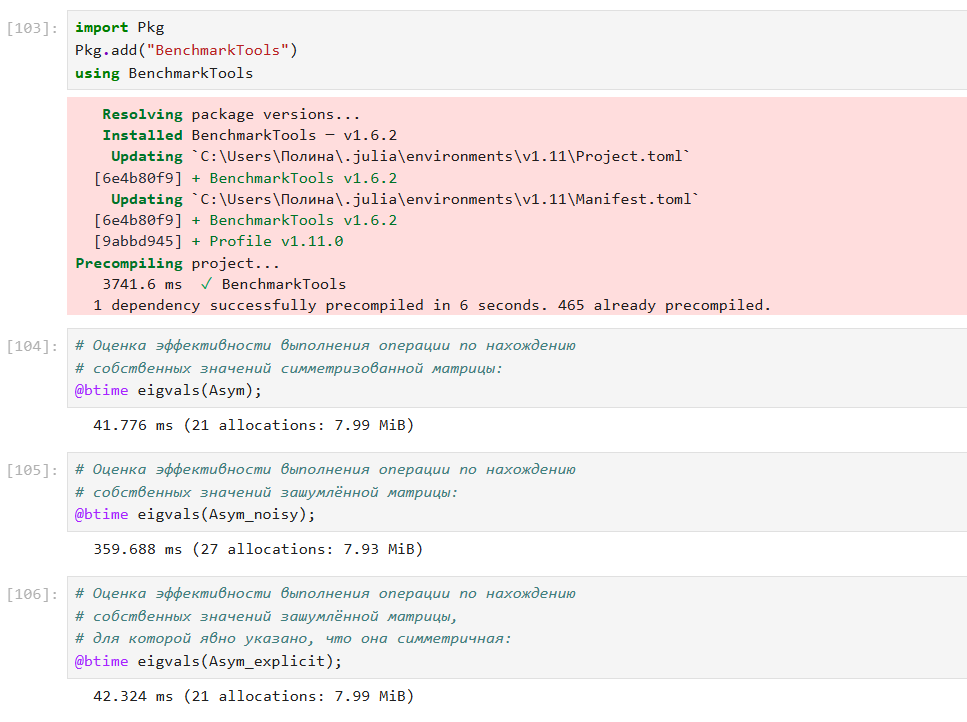
\includegraphics[width=0.7\textwidth,height=\textheight]{image/20.png}
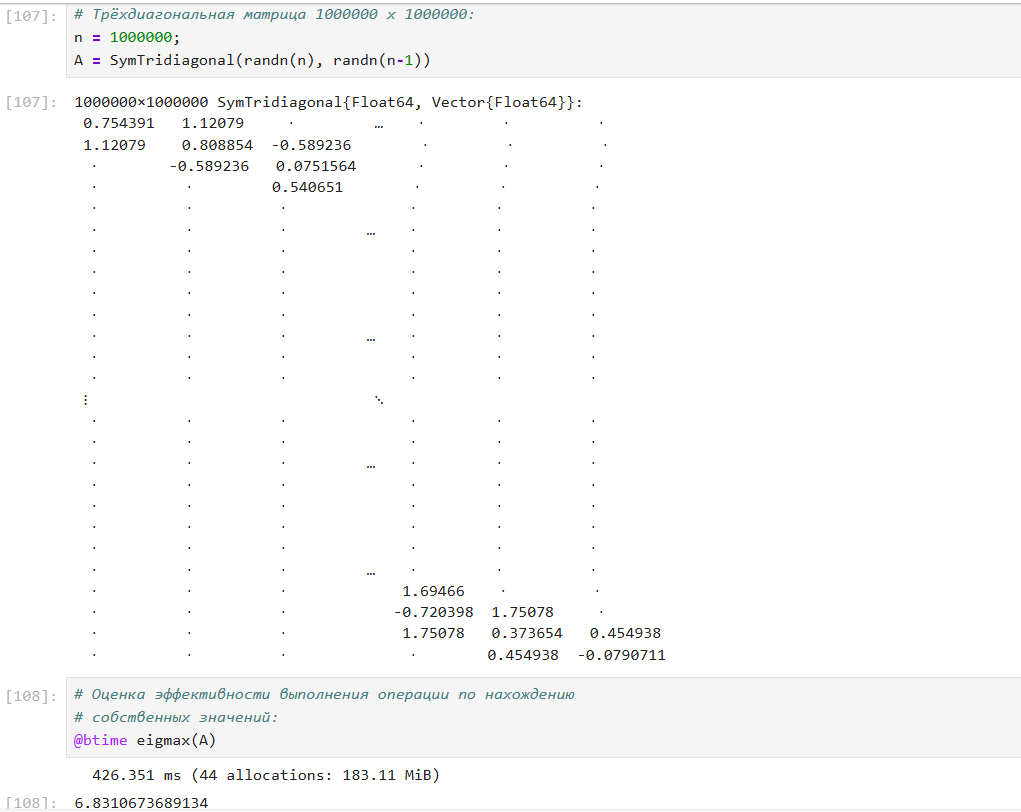
\includegraphics[width=0.7\textwidth,height=\textheight]{image/21.png}

Заполняем карточку инцидента о создании нового подозрительного
пользователя (рис.~\ref{fig-022}).

\begin{figure}

{\centering 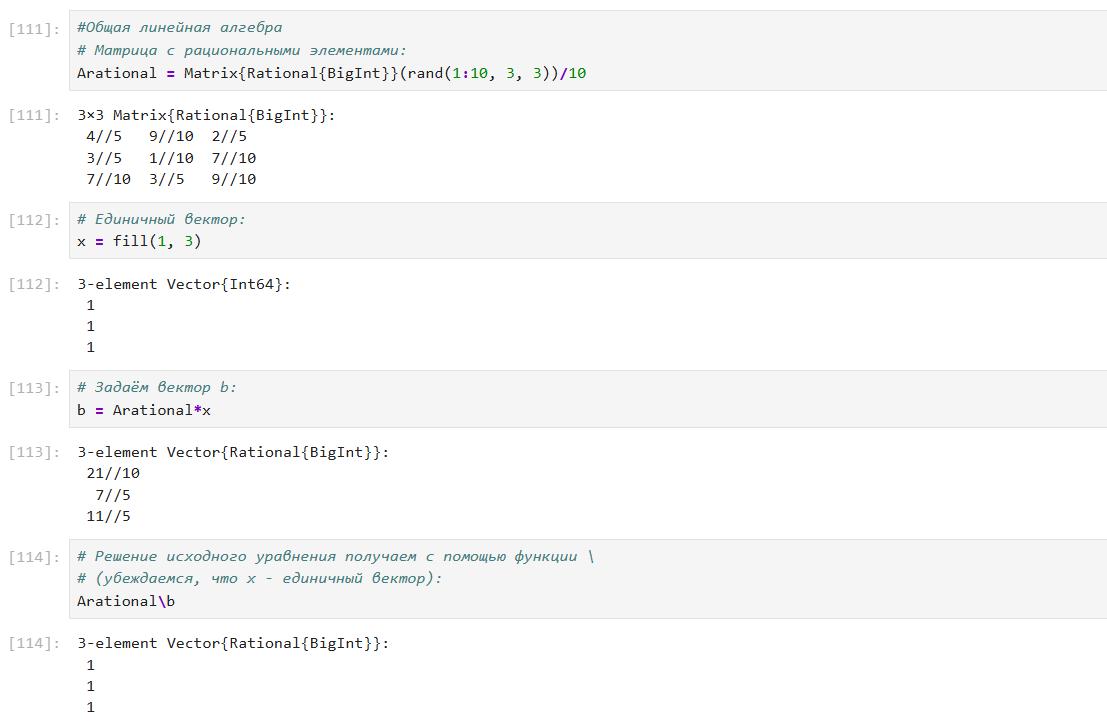
\includegraphics[width=0.7\textwidth,height=\textheight]{image/22.png}

}

\caption{\label{fig-022}Карточка инцидента}

\end{figure}

\hypertarget{ux43eux431ux43dux430ux440ux443ux436ux435ux43dux438ux435-ux442ux440ux435ux442ux44cux435ux439-ux443ux44fux437ux432ux438ux43cux43eux441ux442ux438}{%
\section{Обнаружение третьей
уязвимости}\label{ux43eux431ux43dux430ux440ux443ux436ux435ux43dux438ux435-ux442ux440ux435ux442ux44cux435ux439-ux443ux44fux437ux432ux438ux43cux43eux441ux442ux438}}

\begin{enumerate}
\def\labelenumi{\arabic{enumi}.}
\setcounter{enumi}{5}
\tightlist
\item
  Внутренний нарушитель проводит Blind SQL-инъекцию, получает доступ к
  данным конфиденциального проекта.
\end{enumerate}

Мы видим большое количество SQL запросов, количесвто и постоянство
которых настораживает (рис.~\ref{fig-023}). Так же мы можем видеть
события кражи паролей.

\begin{figure}

{\centering 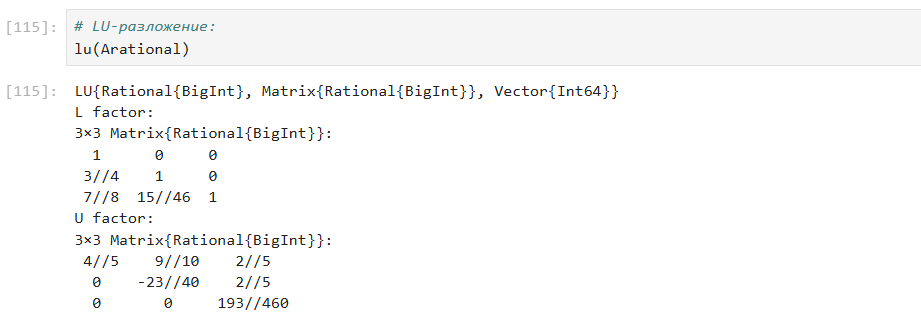
\includegraphics[width=0.7\textwidth,height=\textheight]{image/23.png}

}

\caption{\label{fig-023}SQL-запросы}

\end{figure}

При заполнении карточки уязвимости (\textbf{?@fig-024}) ссылаемся на
гитхаб (\textbf{?@fig-025}).

\hypertarget{ux443ux441ux442ux440ux430ux43dux435ux43dux438ux435-ux443ux44fux437ux432ux438ux43cux43eux441ux442ux435ux439-ux438-ux438ux445-ux43fux43eux441ux43bux435ux434ux441ux442ux432ux438ux439}{%
\chapter{Устранение уязвимостей и их
последствий}\label{ux443ux441ux442ux440ux430ux43dux435ux43dux438ux435-ux443ux44fux437ux432ux438ux43cux43eux441ux442ux435ux439-ux438-ux438ux445-ux43fux43eux441ux43bux435ux434ux441ux442ux432ux438ux439}}

\hypertarget{ux441ux43bux430ux431ux44bux439-ux43fux430ux440ux43eux43bux44c-ux43fux43eux43bux44cux437ux43eux432ux430ux442ux435ux43bux44f}{%
\section{Слабый пароль
пользователя}\label{ux441ux43bux430ux431ux44bux439-ux43fux430ux440ux43eux43bux44c-ux43fux43eux43bux44cux437ux43eux432ux430ux442ux435ux43bux44f}}

Для закрытия уязвимости меняем пароль на более сложный, не содержащийся
в словаре. Для изменения пароля на сервере AD открываем «Active
Directory Users and Computers», меняем пароль для пользователя dev1
(\textbf{?@fig-001}), (\textbf{?@fig-002}).

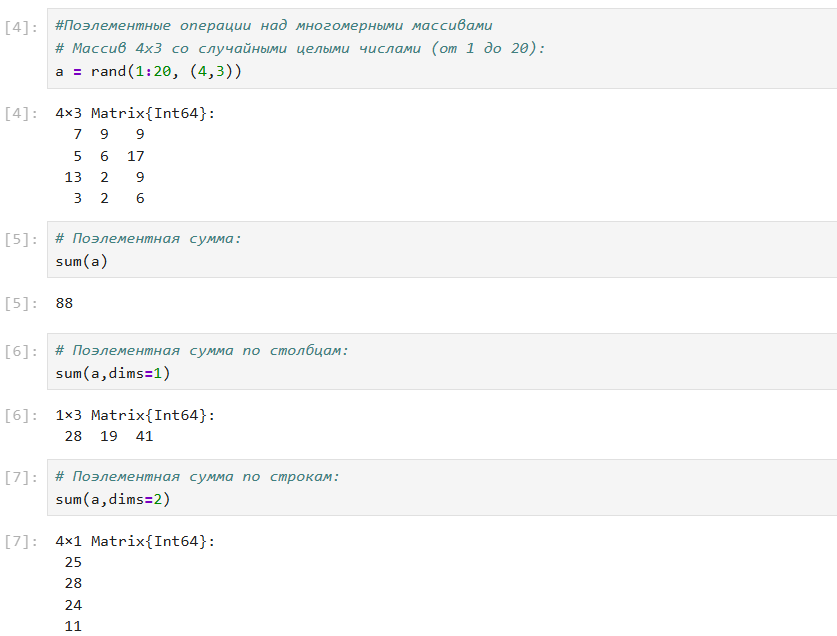
\includegraphics[width=0.7\textwidth,height=\textheight]{image/1.png}
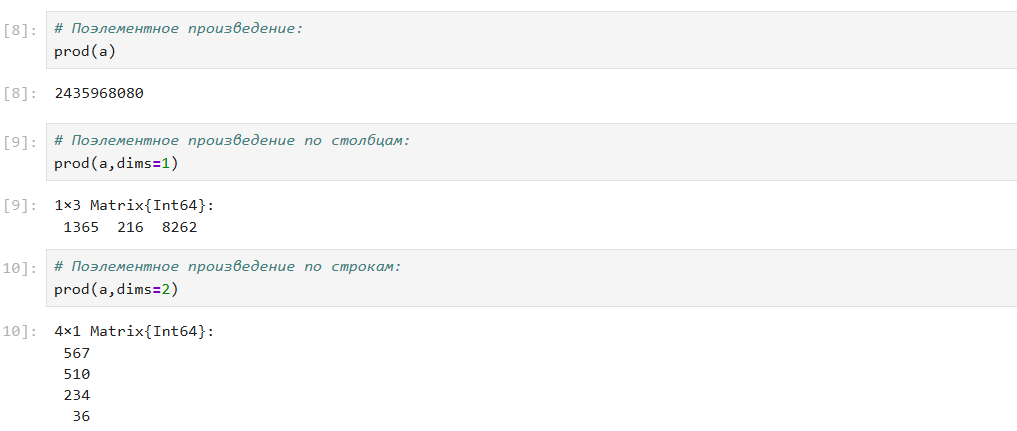
\includegraphics[width=0.7\textwidth,height=\textheight]{image/2.png}

Нарушитель может создать сервис, автоматически запускающий исполняемый
файл, который устанавливает Reverse Shell подключение. Новая задача,
записанная нарушителем, находится на узле Developer 1 (10.10.4.13) в
планировщике задач (\textbf{?@fig-003}).
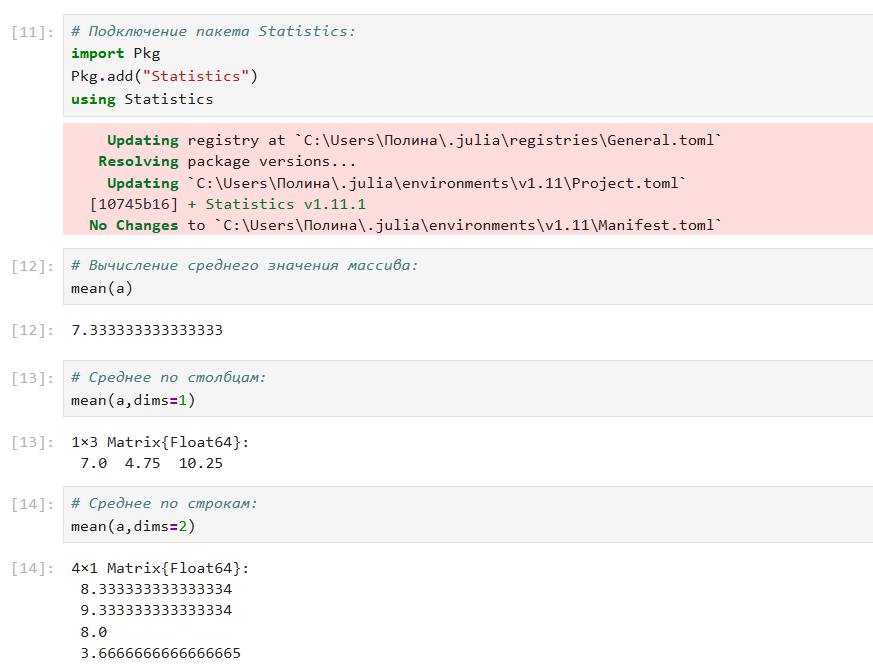
\includegraphics[width=0.7\textwidth,height=\textheight]{image/3.png} Во
вкладке action мы можем обнаружить путь к файлу, что позваляет нам найти
его и удалить.

\hypertarget{ux430ux442ux430ux43aux430-xss}{%
\section{Атака XSS}\label{ux430ux442ux430ux43aux430-xss}}

В Redmine до версии 3.4.11 и 4.0.x до версии 4.0.4 постоянный XSS
существует из-за ошибок форматирования при работе с textile текстом. В
данном сценарии используется для включения REST API для эксплуатации
следующей уязвимости (\textbf{?@fig-004}).
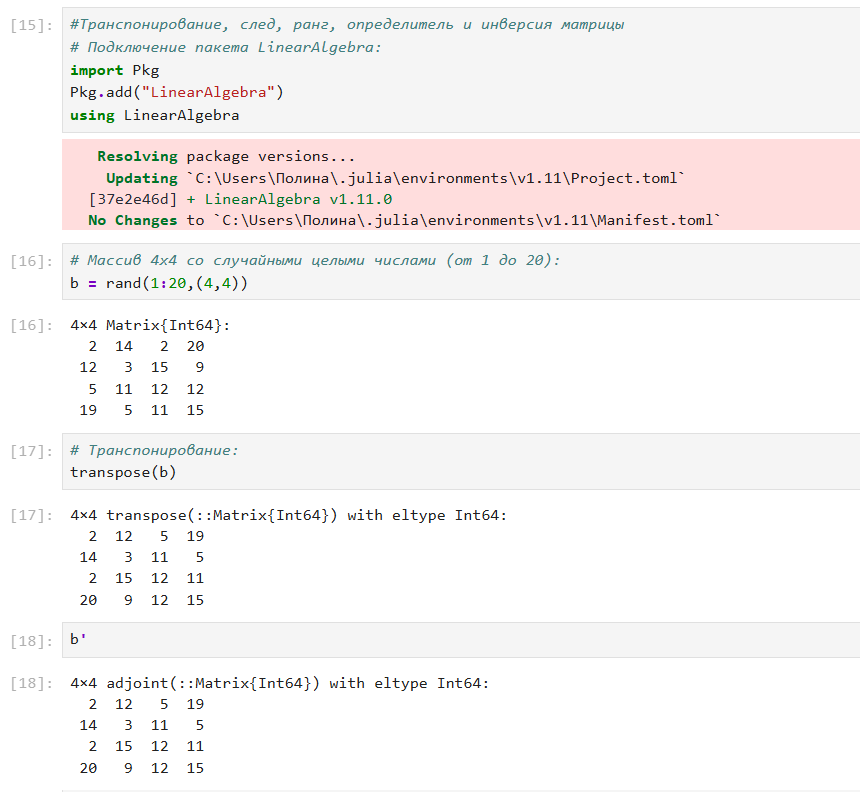
\includegraphics[width=0.7\textwidth,height=\textheight]{image/4.png}

Для устранения этой уязвимости необходимо внести изменения в код
Redmine. Необходимо найти обработку текста wiki-страницы при наличии в
тексте html-тегов. Из описания уязвимости понятно, что необходимо найти
библиотеку для преобразования textile разметки в html. В Redmine за
данное преобразование отвечает Redcloth. Для устранения изменим
следующие строки (\textbf{?@fig-005}).
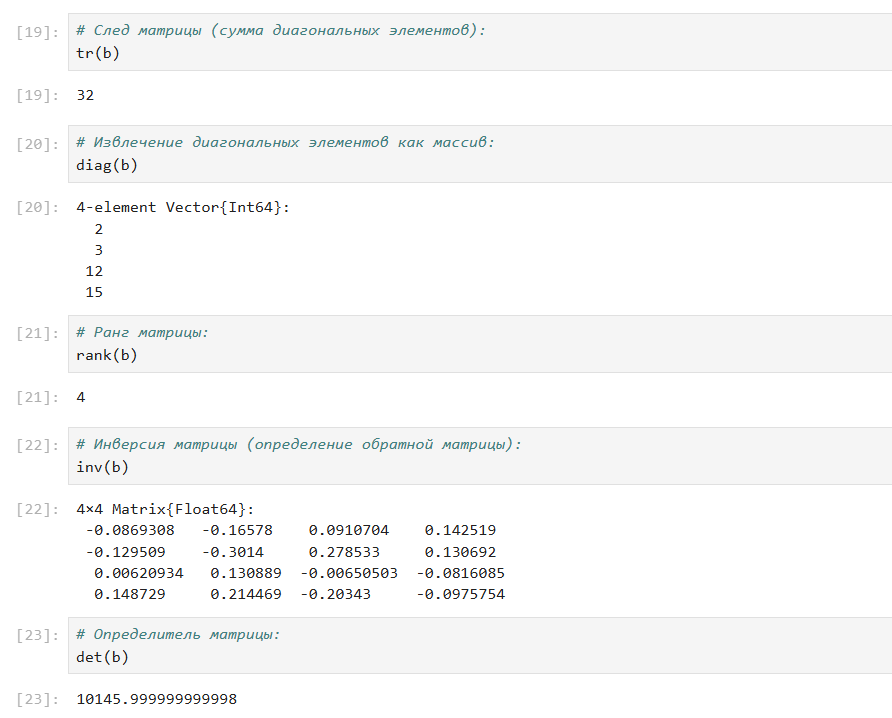
\includegraphics[width=0.7\textwidth,height=\textheight]{image/5.png}

Код, исправляющий уязвимость CVE-2019-17427:

\begin{verbatim}
ALLOWED_TAGS = %w(redpre pre code kbd notextile) 
    def escape_html_tags(text)  
        text.gsub!(%r{<(\/?([!\w]+)[^<>\n]*)(>?)}) do |m| 
            if ALLOWED_TAGS.include?($2) && $3.present? 
                "<#{$1}#{$3}" 
            else 
                "<#{$1}#{'>' unless $3.blank?}" 
            end 
        end 
    end
\end{verbatim}

\begin{figure}

{\centering 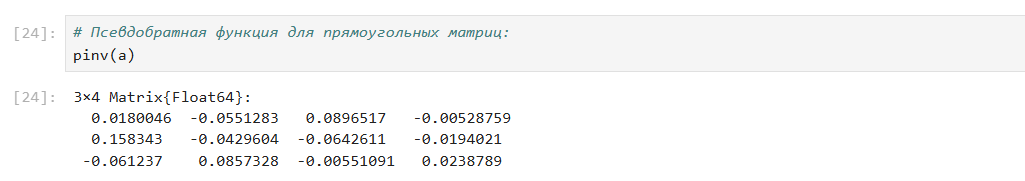
\includegraphics[width=0.7\textwidth,height=\textheight]{image/6.png}

}

\caption{\label{fig-006}Исправления в файле redcloth3.rb}

\end{figure}

После внесения изменений необходимо перезапускаем службу веб-сервера и
видим, что уязвимость успешно устранена (\textbf{?@fig-007}).
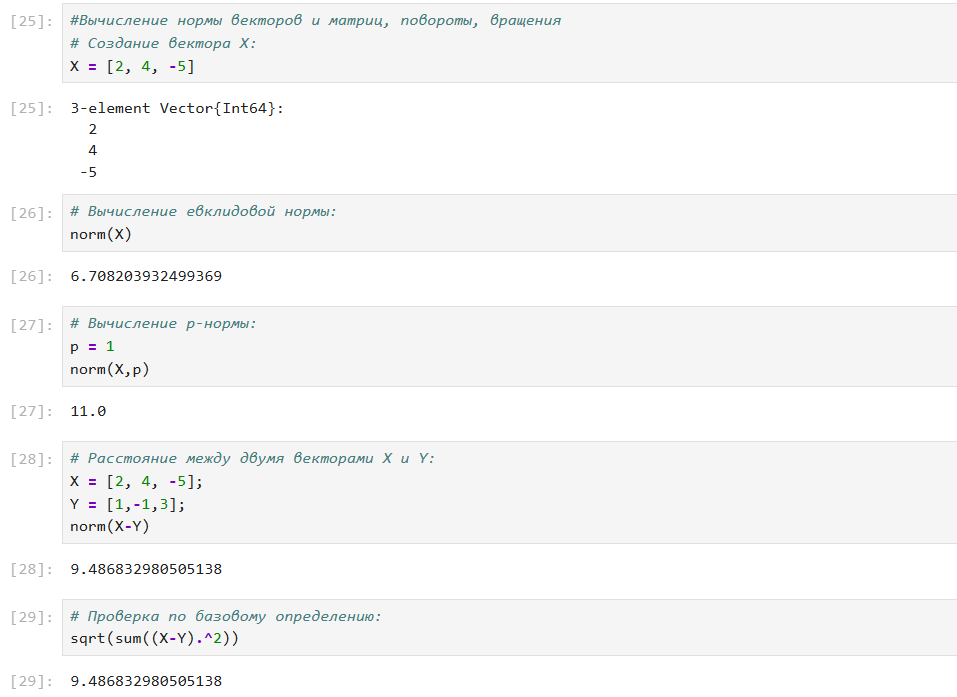
\includegraphics[width=0.7\textwidth,height=\textheight]{image/7.png}

Данная полезная нагрузка заключается в том, что нарушитель создает
пользователя на портале Redmine. Пользователь, обладающий правами
администратора, имеет неограниченный доступ к пользовательской базе. Для
обнаружения добавления нового привилегированного пользователя заходим в
консоль администратора Redmine, переходим в раздел «Administration» --
«Users» и смотрим список существующих пользователей
(\textbf{?@fig-008}).
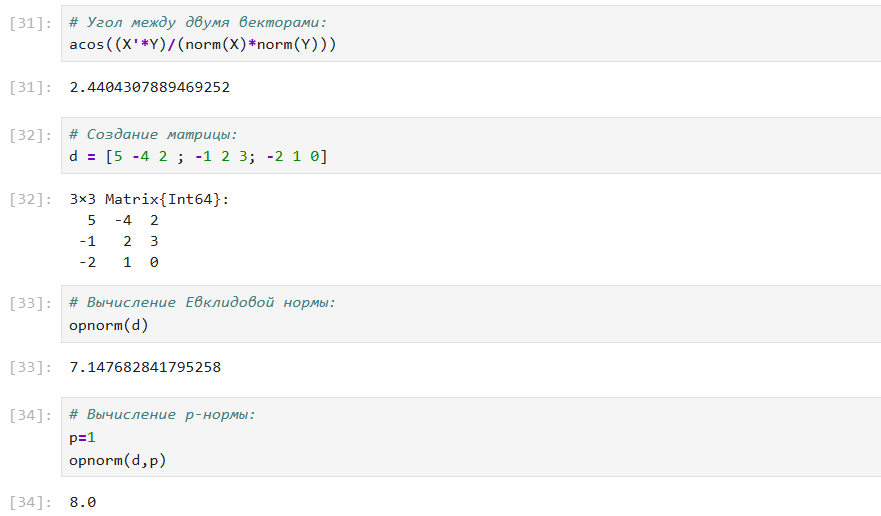
\includegraphics[width=0.7\textwidth,height=\textheight]{image/8.png}
Удаляем пользователя hacker, успешно нейтрализуя последствие Redmine
User.

\hypertarget{blind-sql-ux438ux43dux44aux435ux43aux446ux438ux44f}{%
\section{Blind
SQL-инъекция}\label{blind-sql-ux438ux43dux44aux435ux43aux446ux438ux44f}}

Эксплуатируемая уязвимость -- CVE-2019-18890. В Redmine до версии 3.2.9
и 3.3.x до версии 3.3.10 уязвимость позволяет пользователям Redmine
получать доступ к защищенной информации с помощью сгенерированного
объектного запроса. Уязвимость реализуется посимвольным перебором с
замером времени ответа. В данном сценарии данная уязвимость используется
для получения конфиденциальной информации из БД, минуя разграничение
доступа Redmine. Время прихода пакета является индикатором: при
запоздании пакета -- символ подобран верно, иначе -- перебор
продолжается (\textbf{?@fig-009}).
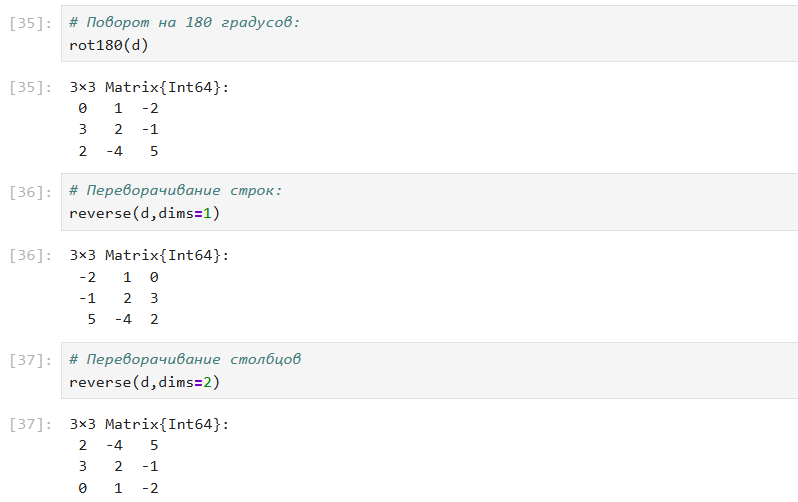
\includegraphics[width=0.7\textwidth,height=\textheight]{image/9.png}

Для устранения этой уязвимости необходимо внести изменения в код
Redmine. Исходя из адреса и запроса следует найти местоположение
скрипта, где происходит обработка параметра subproject\_id. В данном
случае рассмотрен файл query.rb. Вносим изменения в код
(\textbf{?@fig-010}), (\textbf{?@fig-010}) и после перезапуска
веб-сервера уязвимость устраняется.
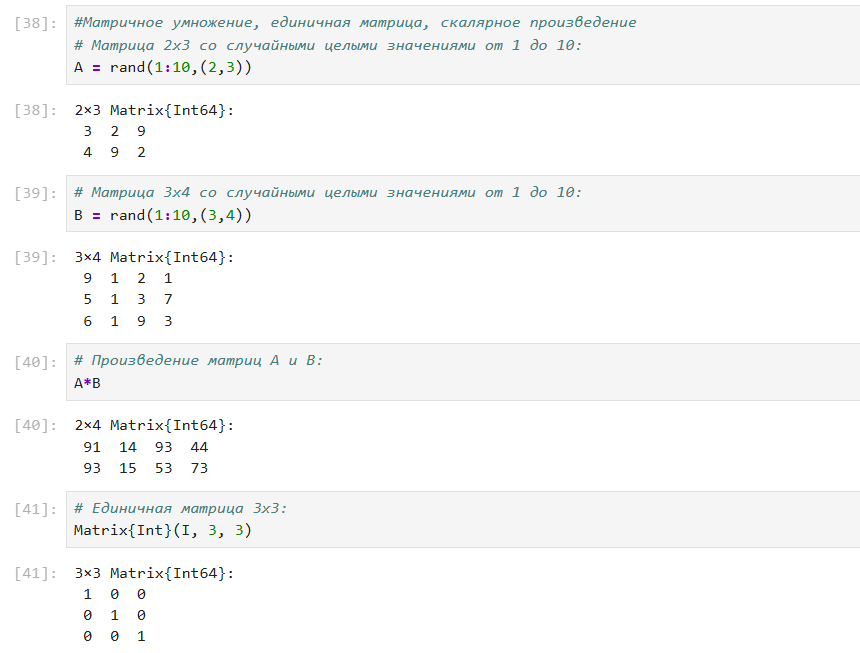
\includegraphics[width=0.7\textwidth,height=\textheight]{image/10.png}
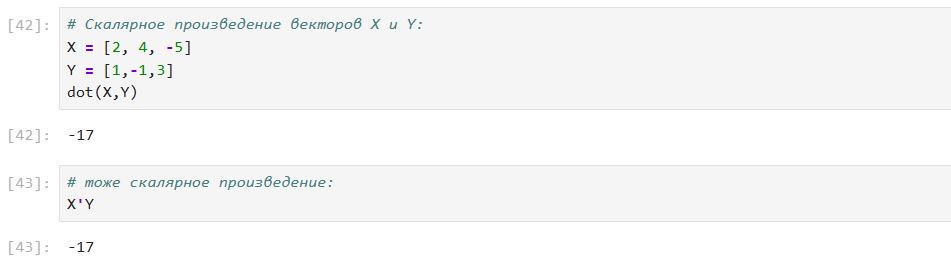
\includegraphics[width=0.7\textwidth,height=\textheight]{image/11.png}


\printbibliography


\end{document}
